\documentclass{standalone}
\usepackage{tikz}
\usetikzlibrary{patterns, positioning}

\begin{document}
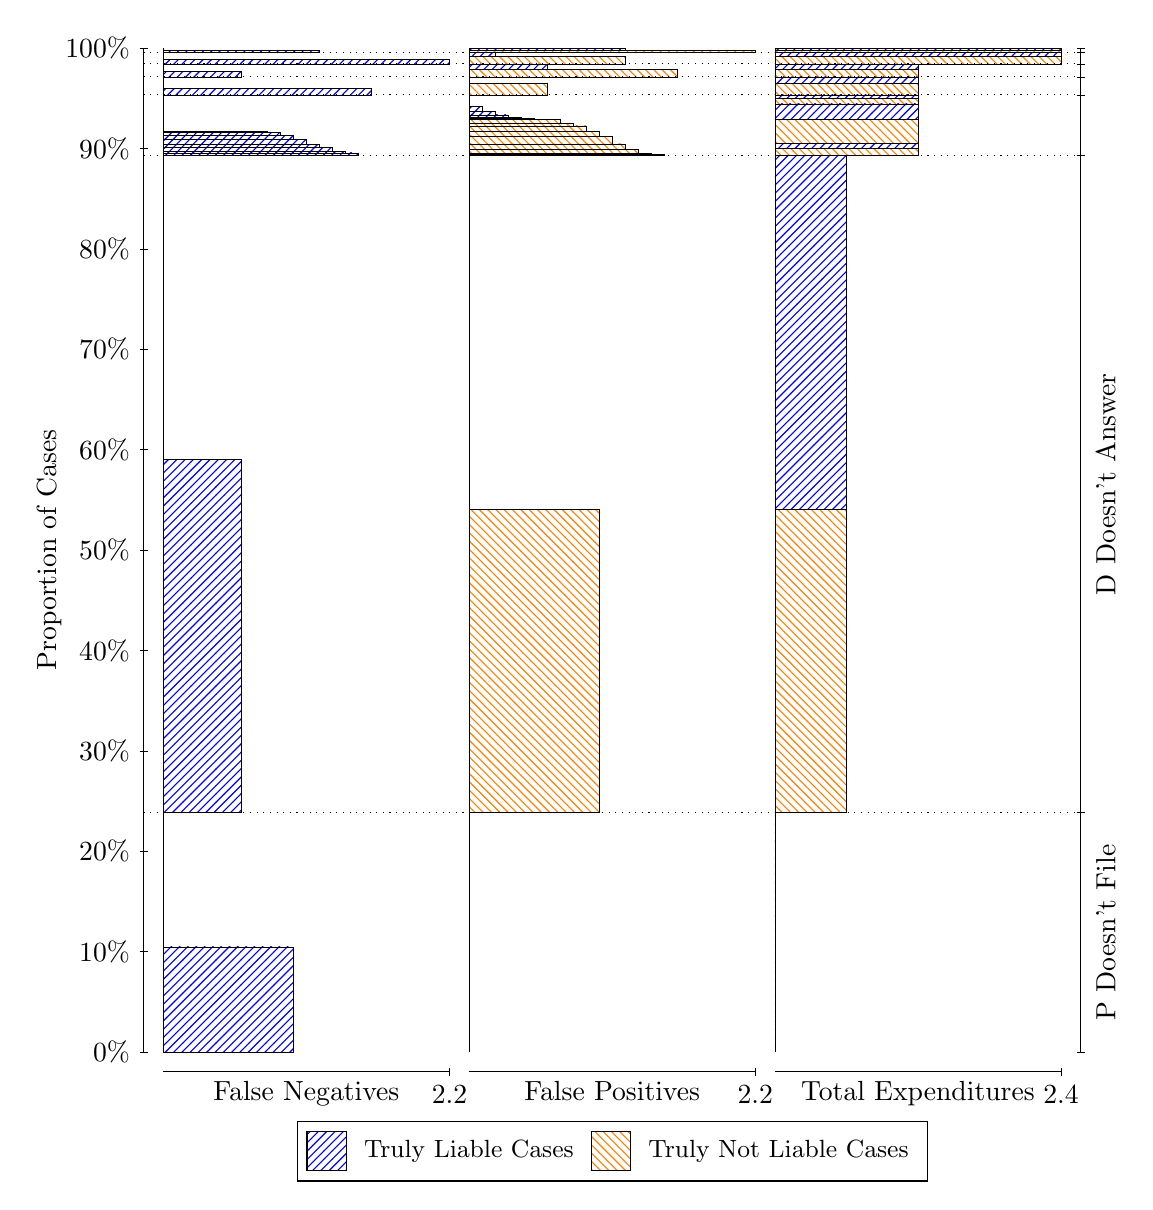
\begin{tikzpicture}
\draw[black, very thin] (1.5,1.75) -- (1.5,14.5);
\node[rotate=90, anchor=center] at (0.3, 8.125) {Proportion of Cases};
\draw[black, very thin] (1.45,1.75) -- (1.55,1.75);
\node[anchor=east] at (1.45, 1.75) {0\%};
\draw[black, very thin] (1.45,3.025) -- (1.55,3.025);
\node[anchor=east] at (1.45, 3.025) {10\%};
\draw[black, very thin] (1.45,4.3) -- (1.55,4.3);
\node[anchor=east] at (1.45, 4.3) {20\%};
\draw[black, very thin] (1.45,5.575) -- (1.55,5.575);
\node[anchor=east] at (1.45, 5.575) {30\%};
\draw[black, very thin] (1.45,6.85) -- (1.55,6.85);
\node[anchor=east] at (1.45, 6.85) {40\%};
\draw[black, very thin] (1.45,8.125) -- (1.55,8.125);
\node[anchor=east] at (1.45, 8.125) {50\%};
\draw[black, very thin] (1.45,9.4) -- (1.55,9.4);
\node[anchor=east] at (1.45, 9.4) {60\%};
\draw[black, very thin] (1.45,10.675) -- (1.55,10.675);
\node[anchor=east] at (1.45, 10.675) {70\%};
\draw[black, very thin] (1.45,11.95) -- (1.55,11.95);
\node[anchor=east] at (1.45, 11.95) {80\%};
\draw[black, very thin] (1.45,13.225) -- (1.55,13.225);
\node[anchor=east] at (1.45, 13.225) {90\%};
\draw[black, very thin] (1.45,14.5) -- (1.55,14.5);
\node[anchor=east] at (1.45, 14.5) {100\%};

\draw[black, very thin] (13.4,1.75) -- (13.4,14.5);
\draw[black, very thin] (13.35,1.75) -- (13.45,1.75);
\node[anchor=west] at (13.35, 1.75) {};
\draw[black, very thin] (13.35,4.7882) -- (13.45,4.7882);
\node[anchor=west] at (13.35, 4.7882) {};
\draw[black, very thin] (13.35,13.133) -- (13.45,13.133);
\node[anchor=west] at (13.35, 13.133) {};
\draw[black, very thin] (13.35,13.906) -- (13.45,13.906);
\node[anchor=west] at (13.35, 13.906) {};
\draw[black, very thin] (13.35,14.134) -- (13.45,14.134);
\node[anchor=west] at (13.35, 14.134) {};
\draw[black, very thin] (13.35,14.298) -- (13.45,14.298);
\node[anchor=west] at (13.35, 14.298) {};
\draw[black, very thin] (13.35,14.444) -- (13.45,14.444);
\node[anchor=west] at (13.35, 14.444) {};
\draw[black, very thin] (13.35,14.5) -- (13.45,14.5);
\node[anchor=west] at (13.35, 14.5) {};

\draw[black, very thin, pattern color=blue, pattern=north east lines] (1.75,1.75) rectangle (3.4015,3.085);
\draw[black, very thin, pattern color=orange, pattern=north west lines] (1.75,3.085) rectangle (1.75,4.7882);
\draw[black, very thin, pattern color=blue, pattern=north east lines] (1.75,4.7882) rectangle (2.7409,9.2768);
\draw[black, very thin, pattern color=orange, pattern=north west lines] (1.75,9.2768) rectangle (1.75,13.133);
\draw[black, very thin, pattern color=blue, pattern=north east lines] (1.75,13.133) rectangle (4.2273,13.167);
\draw[black, very thin, pattern color=blue, pattern=north east lines] (1.75,13.167) rectangle (4.0621,13.188);
\draw[black, very thin, pattern color=blue, pattern=north east lines] (1.75,13.188) rectangle (3.897,13.236);
\draw[black, very thin, pattern color=blue, pattern=north east lines] (1.75,13.236) rectangle (3.7318,13.276);
\draw[black, very thin, pattern color=blue, pattern=north east lines] (1.75,13.276) rectangle (3.5667,13.339);
\draw[black, very thin, pattern color=blue, pattern=north east lines] (1.75,13.339) rectangle (3.4015,13.387);
\draw[black, very thin, pattern color=blue, pattern=north east lines] (1.75,13.387) rectangle (3.2364,13.424);
\draw[black, very thin, pattern color=blue, pattern=north east lines] (1.75,13.424) rectangle (3.0712,13.437);
\draw[black, very thin, pattern color=blue, pattern=north east lines] (1.75,13.437) rectangle (2.9061,13.445);
\draw[black, very thin, pattern color=orange, pattern=north west lines] (1.75,13.445) rectangle (1.75,13.906);
\draw[black, very thin, pattern color=blue, pattern=north east lines] (1.75,13.906) rectangle (4.3924,13.99);
\draw[black, very thin, pattern color=orange, pattern=north west lines] (1.75,13.99) rectangle (1.75,14.134);
\draw[black, very thin, pattern color=blue, pattern=north east lines] (1.75,14.134) rectangle (2.7409,14.205);
\draw[black, very thin, pattern color=orange, pattern=north west lines] (1.75,14.205) rectangle (1.75,14.298);
\draw[black, very thin, pattern color=blue, pattern=north east lines] (1.75,14.298) rectangle (5.3833,14.353);
\draw[black, very thin, pattern color=orange, pattern=north west lines] (1.75,14.353) rectangle (1.75,14.444);
\draw[black, very thin, pattern color=blue, pattern=north east lines] (1.75,14.444) rectangle (3.7318,14.473);
\draw[black, very thin, pattern color=orange, pattern=north west lines] (1.75,14.473) rectangle (1.75,14.5);
\draw[black, very thin, pattern color=orange, pattern=north west lines] (5.6333,1.75) rectangle (5.6333,3.4532);
\draw[black, very thin, pattern color=blue, pattern=north east lines] (5.6333,3.4532) rectangle (5.6333,4.7882);
\draw[black, very thin, pattern color=orange, pattern=north west lines] (5.6333,4.7882) rectangle (7.2848,8.6445);
\draw[black, very thin, pattern color=blue, pattern=north east lines] (5.6333,8.6445) rectangle (5.6333,13.133);
\draw[black, very thin, pattern color=orange, pattern=north west lines] (5.6333,13.133) rectangle (8.1106,13.146);
\draw[black, very thin, pattern color=orange, pattern=north west lines] (5.6333,13.146) rectangle (7.9455,13.162);
\draw[black, very thin, pattern color=orange, pattern=north west lines] (5.6333,13.162) rectangle (7.7803,13.212);
\draw[black, very thin, pattern color=orange, pattern=north west lines] (5.6333,13.212) rectangle (7.6152,13.284);
\draw[black, very thin, pattern color=orange, pattern=north west lines] (5.6333,13.284) rectangle (7.45,13.378);
\draw[black, very thin, pattern color=orange, pattern=north west lines] (5.6333,13.378) rectangle (7.2848,13.438);
\draw[black, very thin, pattern color=orange, pattern=north west lines] (5.6333,13.438) rectangle (7.1197,13.511);
\draw[black, very thin, pattern color=orange, pattern=north west lines] (5.6333,13.511) rectangle (6.9545,13.542);
\draw[black, very thin, pattern color=orange, pattern=north west lines] (5.6333,13.542) rectangle (6.7894,13.594);
\draw[black, very thin, pattern color=blue, pattern=north east lines] (5.6333,13.594) rectangle (6.4591,13.602);
\draw[black, very thin, pattern color=blue, pattern=north east lines] (5.6333,13.602) rectangle (6.2939,13.615);
\draw[black, very thin, pattern color=blue, pattern=north east lines] (5.6333,13.615) rectangle (6.1288,13.652);
\draw[black, very thin, pattern color=blue, pattern=north east lines] (5.6333,13.652) rectangle (5.9636,13.7);
\draw[black, very thin, pattern color=blue, pattern=north east lines] (5.6333,13.7) rectangle (5.7985,13.763);
\draw[black, very thin, pattern color=blue, pattern=north east lines] (5.6333,13.763) rectangle (5.6333,13.906);
\draw[black, very thin, pattern color=orange, pattern=north west lines] (5.6333,13.906) rectangle (6.6242,14.05);
\draw[black, very thin, pattern color=blue, pattern=north east lines] (5.6333,14.05) rectangle (5.6333,14.134);
\draw[black, very thin, pattern color=orange, pattern=north west lines] (5.6333,14.134) rectangle (8.2758,14.226);
\draw[black, very thin, pattern color=blue, pattern=north east lines] (5.6333,14.226) rectangle (6.6242,14.298);
\draw[black, very thin, pattern color=orange, pattern=north west lines] (5.6333,14.298) rectangle (7.6152,14.389);
\draw[black, very thin, pattern color=blue, pattern=north east lines] (5.6333,14.389) rectangle (5.9636,14.444);
\draw[black, very thin, pattern color=orange, pattern=north west lines] (5.6333,14.444) rectangle (9.2667,14.471);
\draw[black, very thin, pattern color=blue, pattern=north east lines] (5.6333,14.471) rectangle (7.6152,14.5);
\draw[black, very thin, pattern color=orange, pattern=north west lines] (9.5167,1.75) rectangle (9.5167,3.4532);
\draw[black, very thin, pattern color=blue, pattern=north east lines] (9.5167,3.4532) rectangle (9.5167,4.7882);
\draw[black, very thin, pattern color=orange, pattern=north west lines] (9.5167,4.7882) rectangle (10.425,8.6445);
\draw[black, very thin, pattern color=blue, pattern=north east lines] (9.5167,8.6445) rectangle (10.425,13.133);
\draw[black, very thin, pattern color=orange, pattern=north west lines] (9.5167,13.133) rectangle (11.333,13.228);
\draw[black, very thin, pattern color=blue, pattern=north east lines] (9.5167,13.228) rectangle (11.333,13.292);
\draw[black, very thin, pattern color=orange, pattern=north west lines] (9.5167,13.292) rectangle (11.333,13.591);
\draw[black, very thin, pattern color=blue, pattern=north east lines] (9.5167,13.591) rectangle (11.333,13.79);
\draw[black, very thin, pattern color=orange, pattern=north west lines] (9.5167,13.79) rectangle (11.333,13.856);
\draw[black, very thin, pattern color=blue, pattern=north east lines] (9.5167,13.856) rectangle (11.333,13.906);
\draw[black, very thin, pattern color=orange, pattern=north west lines] (9.5167,13.906) rectangle (11.333,14.05);
\draw[black, very thin, pattern color=blue, pattern=north east lines] (9.5167,14.05) rectangle (11.333,14.134);
\draw[black, very thin, pattern color=orange, pattern=north west lines] (9.5167,14.134) rectangle (11.333,14.226);
\draw[black, very thin, pattern color=blue, pattern=north east lines] (9.5167,14.226) rectangle (11.333,14.298);
\draw[black, very thin, pattern color=orange, pattern=north west lines] (9.5167,14.298) rectangle (13.15,14.389);
\draw[black, very thin, pattern color=blue, pattern=north east lines] (9.5167,14.389) rectangle (13.15,14.444);
\draw[black, very thin, pattern color=orange, pattern=north west lines] (9.5167,14.444) rectangle (13.15,14.471);
\draw[black, very thin, pattern color=blue, pattern=north east lines] (9.5167,14.471) rectangle (13.15,14.5);
\draw[black, dotted] (1.5,4.7882) -- (13.4,4.7882);
\draw[black, dotted] (1.5,13.133) -- (13.4,13.133);
\draw[black, dotted] (1.5,13.906) -- (13.4,13.906);
\draw[black, dotted] (1.5,14.134) -- (13.4,14.134);
\draw[black, dotted] (1.5,14.298) -- (13.4,14.298);
\draw[black, dotted] (1.5,14.444) -- (13.4,14.444);
\draw[black, very thin] (1.75,1.5) -- (5.3833,1.5);
\node[anchor=north] at (3.5667, 1.5) {False Negatives};
\draw[black, very thin] (5.3833,1.45) -- (5.3833,1.55);
\node[anchor=north] at (5.3833, 1.45) {2.2};

\draw[black, very thin] (5.6333,1.5) -- (9.2667,1.5);
\node[anchor=north] at (7.45, 1.5) {False Positives};
\draw[black, very thin] (9.2667,1.45) -- (9.2667,1.55);
\node[anchor=north] at (9.2667, 1.45) {2.2};

\draw[black, very thin] (9.5167,1.5) -- (13.15,1.5);
\node[anchor=north] at (11.333, 1.5) {Total Expenditures};
\draw[black, very thin] (13.15,1.45) -- (13.15,1.55);
\node[anchor=north] at (13.15, 1.45) {2.4};

\node[black, centered, rotate=90] at (13.72, 3.2691) {P Doesn't File};
\node[black, centered, rotate=90] at (13.72, 8.9607) {D Doesn't Answer};






\draw (7.449999999999999,1.5) node[draw=none] (baseCoordinate) {};
\begin{scope}[align=center]
        \matrix[scale=0.5, draw=black, below=0.5cm of baseCoordinate, nodes={draw}, column sep=0.1cm]{
            \node[rectangle, draw, minimum width=0.5cm, minimum height=0.5cm, pattern=north east lines, pattern color=blue] {}; &
            \node[draw=none, font=\small] (B) {Truly Liable Cases}; &
            \node[rectangle, draw, minimum width=0.5cm, minimum height=0.5cm, pattern=north west lines, pattern color=orange] {}; &
            \node[draw=none, font=\small] (B) {Truly Not Liable Cases}; \\
            };
\end{scope}

\end{tikzpicture}
\end{document}